\documentclass{article}
\usepackage{graphicx}
\usepackage{subfigure}
\usepackage{caption}
\usepackage{lipsum}
\usepackage{amsmath}
\usepackage{amsthm}
\usepackage{geometry}
\usepackage{amsfonts}
\usepackage{ragged2e}
\usepackage{amssymb}
\usepackage{mathrsfs}
\usepackage{enumitem}
\geometry{
 a4paper,
 total={170mm,257mm},
 left=20mm,
 top=20mm,
 }
\usepackage[utf8]{inputenc}

\title{Tarea 2 Metodos Computacionales}
\author{Luis Carlos Mantilla 201631487}
\date{Julio 2019}

\begin{document}

\maketitle

\section*{Punto 1}

La idea de este ejercicio es lograr unir dos im\'agenes de tal manera que vista de cerca sea una imagen y vista de lejos sea la otra imagen. Esto lo podemos hacer tomando el espectro de Fourier de ambas im\'agenes y tomar las frecuencias altas de una y las bajas de la otra y finalmente sumar ambas. En nuestro caso, esta suma se hace con distintos pesos para resaltar m\'as algunos detalles. 

\subsection*{Im\'agenes a unir}
Las dos im\'agenes que vamos a unir son las siguientes:
\begin{figure}[!htbp]
  \centering
  \subfigure[Seria]{
    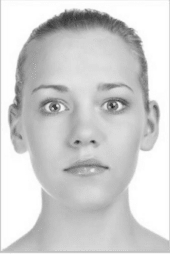
\includegraphics[width=0.23\textwidth]{cara_02_grisesMF.png}%
    }\hspace{0.2cm}
    \subfigure[Sonriendo]{
    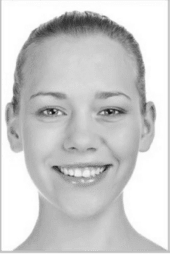
\includegraphics[width=0.228\textwidth]{cara_03_grisesMF.png}%
  }  
  \caption{Caras a unir}
\end{figure}

\subsection*{Transformada de Fourier Caras Separadas}
La transformada de Fourier de cada imagen se realiza con los paquetes de numpy de fft. Se obtienen los siguentes resultados:
\begin{figure}[!htbp]
 \centering
  \includegraphics[scale=0.5]{TransformadaAmbasCaras.png}
\end{figure}

Podemos filtrar con una función Sigmond para obtener una funci\'on escal\'on suavizada
\begin{equation*}
    f(x) = \frac{1}{1+ \exp(-15x)}
\end{equation*}

\subsection*{Transformada Inversa de Fourier Caras Separadas}
Despu\'es del filtrado, usando los paquetes de numpy, se tienen las siguientes caras:
\begin{figure}[!htbp]
  \centering
  \subfigure[Seria]{
    \includegraphics[width=0.55\textwidth]{CaraPasaAltas.png}%
    }\hspace{0.05cm}
    \subfigure[Sonriendo]{
    \includegraphics[width=0.55\textwidth]{CaraPasaBajas.png}%
  }  
  \caption{Caras despues del filtrado}
\end{figure}

\subsection*{Transformada de Fourier Caras Juntas}
Para juntar ambas caras, usamos el la funci\'on Sigmond desplazada y la multiplicamos por las frecuencias de la imagen. Para el filtro pasa altas (la cara seria) desplazamos la funci\'on Sigmond $24$ unidades y se invierte. Para el filtro pasa bajas (la cara sonriendo) desplazamos la funci\'on Sigmond $27$ unidades. Despu\'es de multiplicados los espectros de Fourier por estas funciones, al sumarlos obtenemos el siguiente espectro de Fourier:
\begin{figure}[!htbp]
 \centering
  \includegraphics[scale=0.8]{TransformadaHibrida.png}
  \caption{Espectro de Fourier para la suma de im\'agenes filtradas}
\end{figure}
\subsection*{Transformada Inversa de Fourier Caras Juntas}

Finalmente, al juntar ambas im\'agenes y ajustar un poco sus tama\~nos para que los ojos en ambos casos se sobrepongan se obtiene el siguiente resultado. 

\begin{figure}[!htbp]
 \centering
  \includegraphics[scale=0.8]{CaraHibrida.png}
  \caption{De cerca se ve una cara seria y de lejos una cara sonriendo}
\end{figure}

\pagebreak

\section*{Punto 2}

\subsection*{M\'etodos para solucionar el problema}
La idea de este ejercicio es solucionar la ecuaci\'on diferencial de segundo orden de la fuerza gravitacional entre dos masas para una condici\'on inicial de $\Vec{v} = (-6.35,0.606) $[AU]/[YR] y $\Vec{r} = (0.1163,0.9772)$ [AU].
\begin{equation*}
   m \frac{d^2 \Vec{r}}{dt^2} = -\frac{GMm }{r^2} \hat{r}
\end{equation*}

Esto lo podemos descomponer en dos ecuaciones de primer orden para poder solucionarlas simult\'aneamente

\begin{equation*}
    \frac{d \Vec{v}}{dt} = -\frac{GM }{r^2} \hat{r}
\end{equation*}

y

\begin{equation*}
    \frac{d\Vec{r}}{dt} = \Vec{v}
\end{equation*}

Solucionamos las siguientes ecuaciones con distintas elecciones de dt para aproximar las derivadas temporales con 3 m\'etodos num\'ericos: Euler, RungeKutta de 4to Orden y LeapFrog. Se solucionan con los siguientes distintos valores de dt. 
\begin{itemize}
    \item $dt1=0.0006283 $[YR] $= 19814.0688$[s]
    \item $dt2 = 0.006283$ [YR] $= 198140.688$[s]
    \item $dt3 = 0.12566$ [YR] $= 3962813.76$[s]
\end{itemize}

Esto con el fin de dar aproximadamente $10000$ pasos por orbita con el primer $dt$, $1000$ pasos con el segundo $dt$ y $500$ pasos con el tercer $dt$.


Las siguientes gr\'aficas est\'an organizadas de la siguiente manera: La primera fila utiliza el m\'etodo de Euler, la segunda fila el m\'etodo de RungeKutta de cuarto orden y la tercera fila el m\'etodo de LeapFrog. La primera columna utiliza el $dt1$ para calcular la evoluci\'on temporal del sistema, la segunda columna el $dt2$ y la tercera columna el $dt3$.

\textbf{NOTA SOBRE UNIDADES: }Dado que se trabaja con unidades de Unidades Astron\'omicas [AU], Masas Solares [MS] y a\~nos [YR], los valores de energ\'ias cin\'eticas, potenciales, totales y los momentos angulares se  multiplican  por un factor de $100000$ para cuantificar con mayor facilidad las fluctuaciones en las gr\'aficas.
\subsection*{Posiciones Orbitales}

\begin{figure}[!htbp]
 \centering
  \includegraphics[width=1\textwidth]{posiciones.png}
  \caption{Orbitas descritas por distintos m\'etodos en 20 a\~nos }
\end{figure}
Para hallar las posiciones orbitales necesitamos solucionar la ecuaci\'on de movimiento anteriormente descrita. Se simula un total de 20 a\~nos con cada m\'etodo.
Se puede apreciar que el m\'etodo de Euler es el que peor simula esta situaci\'on dado a la forma como aproxima (con Forward Difference) y el que mejor simula es RungeKutta (aunque LeapFrog tambi\'en hace un muy buen trabajo).

\subsection*{Momento Angular}

\begin{figure}[!htbp]
 \centering
  \includegraphics[width=1\textwidth]{angularMomentum.png}
  \caption{Momento Angular}
\end{figure}

El momento angular es una cantidad f\'isica conservada
\begin{equation*}
    \Vec{L} = \Vec{r} \times \Vec{p}
\end{equation*}
Vemos que los m\'etodos de RungeKutta y LeapFrog mantienen muy bien esta cantidad. El m\'etodo de Euler causa un aumento significativo del Momento Angular, en el tercer $dt$ se llega casi a duplicar el momento inicial despu\'es de $20$ a\~nos de evoluci\'on temporal. En las gr\'aficas, dado que las componentes z de nuestra posici\'on y momento lineal son nulas, la direcci\'on del momento angular ser\'a \'unicamente en direcci\'on z, por ende solo se grafica su magnitud (escalada por $100000$). 

\subsection*{Energ\'ia Potencial}


Se sabe que la energ\'ia potencial gravitacional de un sistema de dos masas est\'a dada por 
\begin{equation*}
    U(\Vec{r}) = -\frac{GMm}{r} 
\end{equation*}

\begin{figure}[!htbp]
 \centering
  \includegraphics[width=1\textwidth]{EnergiaPotencial.png}
  \caption{Energ\'ia Potencial}
\end{figure}

En una orbita el\'iptica como lo es la tierra, uno debería esperar un comportamiento sinusoidal en la energ\'ia potencial. Los tres m\'etodos presentan comportamientos sinusoidales pero el m\'etodo de Euler presenta un aumento en energ\'ia potencial, indicando que la orbita est\'a aumentando, lo cual se sabe que est\'a mal.

\subsection*{Energ\'ia Cin\'etica}

Se sabe que la energ\'ia cin\'etica de una masa con velocidad $\dot{\Vec{r}}$ es
\begin{equation*}
    K(\dot{\Vec{r}}) = \frac{1}{2}m \dot{r}^2
\end{equation*}

De igual manera que la energ\'ia potencial, esperamos para una orbita el\'iptica un comportamiento sinusoidal en la energ\'ia cin\'etica. Dado que en una orbita el\'iptica entre m\'as lejos se encuentre del sol (una mayor energ\'ia potencial) se tendr\'a una velocidad menor y viceversa entre m\'as cerca se encuentre del sol, esperamos encontrar que este comportamiento sinusoidal sea opuesto a aquel de la energ\'ia potencial. Esto se ve de manera clara para los m\'etodos de RungeKutta y LeapFrog, no tanto para el m\'etodo de Euler. 

\begin{figure}[!htbp]
 \centering
  \includegraphics[width=1\textwidth]{EnergiaCinetica.png}
  \caption{Energ\'ia Cin\'etica}
\end{figure}



\subsection*{Energ\'ia Total}


La energ\'ia total del sistema es una cantidad conservada.
\begin{equation*}
    E(\Vec{r}) = U(\Vec{r}) + K(\dot{\Vec{r}})
\end{equation*}
\begin{figure}[!htbp]
 \centering
  \includegraphics[width=1\textwidth]{EnergiaTotal.png}
  \caption{Energ\'ia Total (Cin\'etica + Potencial)}
\end{figure}

Vemos que la energ\'ia total pr\'acticamente se conserva cuando implementamos el m\'etodo de RungeKutta y LeapFrog, se mantienen muy estables. En contraste, el m\'etodo de Euler presenta grandes fallos, y la energ\'ia no se esta conservando, aumenta en cada paso. En el caso de la energ\'ia cin\'etica y la energ\'ia potencial, es claro ver que comienzan y terminan en puntos opuestos y presentan comportamientos peri\'odicos, de tal manera que la suma es constante. Este comportamiento peri\'odico ocurre cuando la tierra esta en el Perihelio o en el Afelio.





\end{document}


